\documentclass[conference]{IEEEtran}

\renewcommand\IEEEkeywordsname{Keywords}
\usepackage{biblatex}
\usepackage{graphicx}
\usepackage{mathtools}

\DeclarePairedDelimiter\floor{\lfloor}{\rfloor}


\begin{document}

\title{Identification of Anamalous Users in Twitter based on users behaviour using Artificial Neural Networks}

\author{
\IEEEauthorblockN{Dr. Kiran K, C. Manjunatha, Dr. P. Deepa Shenoy, Dr. Venugopal K R}	
\IEEEauthorblockA{
Dept. of Computer Science and Engineering\\
University Visvesvaraya College of Engineering\\
Bangalore Karnataka\\
E-mail:manjunathagee@gmail.com
E-mail:kirank.uvce@bub.ernet.in
}

}

\maketitle

\begin{abstract}

With increased number of users in OSN such as Facebook, Twitter, Instagram etc as lead to privacy and security concerns, in this paper we proposed a behavioral based risk assessment method which will help to identity Social bots and compromised accounts in Twitter by leveraging the Neural Networks.
Our solution can detect unusual accounts based on the users writing style such as time of tweeting, language used for writing tweet, frequency of tweeting, etc. This way if the writing style of the user changes 
from what is considered to be normal will flag the user as risky, and the OSN admin can formulate strategies to overcome the same. Experiments were performed 
on the real world dataset extracted from twitter. Experiments results shows tremendous accuracy in identifying social bots and  only few tweets are required to identify that the account has been compromised or not.

\end{abstract}

\begin{IEEEkeywords}

Anamoly Detection, Compromised Account Detection, Neural Networks, Social Bots, Twitter.

\end{IEEEkeywords}

\section{Introduction}

Online Social Network (OSN) is a communication media where people share their thoughts, emotions and opinion about any subjects. At present, Social networks like facebook, twitter, instagram etc are exposed
into area of information and research like Customer Relationship Management (CRM) and Opinion Mining (OM). Information extracted from Social Networks like Twitter and Facebook are extremely valuable for research
and marketing companies, Text Mining, and public opinion organisations.
In Social Network, millions of opinions are expressed with simplicity, unbiased and easy content comprehension. Because of this reason, dataset of Online Social Networks are valuable for decision making on 
business intelligence, marketing research,  image monitoring, and stock market prediction.

The wide popularity of Online Social Networks such as Facebook, twitter, instagram etc and their ease of use have resulted in the compromise of their privacy and security of the users. 

Twitter is a microblogging and social networking  platform which enables registered users to read, write, retweet and reply etc to other users with messages, so-called tweets.
According to a research \footnote{https://www.statista.com/statistics/282087/number-of-monthly-active-twitter-users/} the worldwide population of monthly active users is 336 million for the first quarter of 2018 and the number keeps increasing. A new study at \footnote{https://www.cnbc.com/2017/03/10/nearly-48-million-twitter-accounts-could-be-bots-says-study.html} suggests 
that nearly 48 million twitter accounts are social bots, which means accounts controlled by software, algorithmically generating content to influence and target specific category of audience.

Many social bots perform many useful automated tasks such as creating scheduled news posts etc. However there is an incrased number of social bots which are created to perform malicious activites such as to support political agenda, promote terrorist activities for recuritment, to propogate fasle rumors and conspiracy theories. 

\section{Data Extraction}

Our data extraction process focused on extracting real world data with the help of a pyhton library called 'tweepy'. It starts with a given single user and in order to keep data extraction in close circle first we queried all the friends from user profile and for each user will extract features like user id,tweet id, time of tweet, langulage used for sending tweet, source, friends count, followers count, favorite count, user longevity.

For instance if user A is given, will extract 45 friends from the user profile, so the total number of users are 46, and for each of this 46 users will extract all teh features from there public profile and we repeated this process for 3 months starting from Feb 2018. Care is taken to avoid repetative data extraction i.e if the data is already extracted for a user will skip the data extraction for the next time.

\section{Types of Attacks in OSN}
In general, attackers use OSN to propogate false agenda, extract personal information and even convence the users to provide sensitive financial data llike credit card details etc, they also convence users to click on a malicious links which will propagate the malicous contents on users wall. Below will take a look at well known types of attacks which happends in majority of OSN.

\subsection{Sybil Attack}
Sybil attack are the most common type of attack in majority of the OSNs, In order to launch sybils a malicious users has to create multiple fake accounts in order to gain his identity by targeting a particular community and starts sending friend requests and once friend requests are accepted, over a period of time the attacker will convence the users to buy fake online products, provide credit card details, bank details and even convenence the users to progate the malicious links onto their wall.

\subsection{Compromised Accounts}
Compromised accounts are the real users who as lost their account credentials partially or fully, attackers user cross-site scripting to steal user credentials by manipulating the login forms and DOM. Once the attacker get hold of the original credentials, users friends are targeted to promote malicious content very easily. Compromised account detection is not simple since the user is having legitimate relationship with his/her friends and followers over a period of time. Howerver by monitering users writing style over a period of time and by comparing with the new contents,compromised accounts can be detected.

\subsection{Socware attacks}
Socware is derived from two words \textbf{soc}ial mal\textbf{ware} - \textbf{socware}, here attackers create malicious links to lure people to click on it to acquire user credentials, spread the malicious links on the users wall or to support a particular false agenda. upon clicking link users are take to some inappropriate sites or can even run the virus on users machine to steal sensitive information.

\subsection{Creepers attacks}
Creepers are real users who use OSN in inappropriate ways, for instance they sometimes sell their account temporeraly to some third party to promote advitisements, to promote some false agenda. By observing the the types of links the user posts over a period of time and by analysing them against blocklisted urls creepers accounts can be identified.

\subsection{Identity Cloning}
Identity cloning happens when an attacker makes an exact replica of an existing users account by collecting there public profile details and starts sending requests to their firnds in their timeline and once the requests are accepted over a period time the attacker convences the users to buy online fake product, post fake malicious links on their wall etc.
By comparing the public profile amongst the close friends circle identiy cloning can be identified.

\subsection{Cyber bullying}
This is the common type of attack in OSN where an attacker repeatedly sends hurtfull messages, shares private picture or videos of the victims(usually teenagers and children) and harass them. One way to identify this type of attack is to monitor the users messages if there are more incoming messages without any likes or shares or replies then there is a high probablity that the receiver is a victim of the attack.

\section{Releated Work}
Many approaches have been proposed by authors over a period of time in order to detect aforementioned types of attackes, SVM(Support Vector Machine) classifiers are used to seggregate the user posts based on spam keyword score to identify the SocWare attack \cite{1}, Sybil detector apps were developed for RenRen(Chinese OSN) using regression by segregating the sybil accounts with the normal accounts based on user behaviour \cite{2} \cite{3} COMPA app generated for facebook compares every message generated with the history of messages to flag of compromised accounts, FRAppE generated for facebook successfully identifies the malicious apps by analysing the permissions which the apps requires during authentiction \cite{4}


Many of the previosly proposed work on detecting bots are achieved by implying the full access to all data.These collected data will be clustered according to the behavioral patterns of users (Wang et al. 2013a). For instance, Beutel et al. decomposed event data in time, user, and activity dimensions to extract similar behaviors (Beutel et al. 2013). These techniques are useful to identify coordinated large-scale attacks directed at a common set of targets at the same time, but accounts with similar strategies might also target different groups and operate separately from each other.


One of the study on detecting the spam twitter was done by the author Yardi et al. \cite{20} in the year 2010. They proposed a behavioral patterns to detect the accounts which are purely created to send the spam. But they were able to find only small diferences compared to normal accounts. Twitter accounts also reacts to the spam problem on social network. It is constantly trying to optimise its solutions to redue the spammers. Another work done by Thomas et al. \cite{21} proposed the method to analyse the accounts suspended by Twitter and they found out that 77 percent of the spam accounts detected by Twitter is deleted within 24 hours and 92 percent within three days. However, many of the celebrities controls over thousands of Twitter accounts and creates new accounts to replace the suspended account. 

Many of the research was done on spam on Twitter over many of the years. N.N. Patil, and N.S. Gawale proposed a system to detect URLs on Twitter which contains malicious content\cite{6}. One more method was proposed by Chen et al. \cite{23} which evaluated the ability of spam detection by using various machine learning algorithms. They found that Naive Bayes and SVM tend to outperform other classifiers on spam detection.

However, the accounts which are hacked are not created for sending spam and therefore they are lot harder to prevent. There are less research done on these compromised accounts. G. Specht and  E.Zangerle proposed a method to find classified tweets about being hacked,
based on the behaviour and reaction of the original user \cite{23}. One more proposal was done by Thomas et al. \cite{15} will show the impact of the compromised account by exposing the threat of criminal account hijacking and the damage they can do. The research done by Egele et al. [5]  has the same approach as this study. They proposed a tool that identifies compromised accounts on Facebook and Twitter. The tool considers 6 features into account. Each feature has its own weight, which are determined  by the labelled training dataset of Facebook and Twitter. The weights for the Twitter features were found to be as follows:Personal Interaction (1.4),  Source (3.3), Hour of Day (0.88), Domain (0.96), Topic (0.39) and  Language (0.58). The propsed method was able to detect compromised accounts with a false positive of 3.6 percent.

\section{Features Desciption}
\label{featureDescription}
In this section we will discuss the derived features which are used to train the Artifical Neural Network.

\subsection{FriendShip Ratio}
The normal behaviour of any user in any OSN is that when he/her creates a new account the rate at which he makes friends is limited, by considering the rate at which an user sends a friends request we can easily identify the account is a bot or not. The research done by Zhi Yang, Christo Wilson clearly shows that the bots are aggressive in establishing new connection with strangers within less span of time. We assume that if an user successfully establishes large connections within less span of time then its not a normal behaviour.

\begin{equation}
	 FR (U) = \frac{|Friends(U)|}{User Longevity} \\
\end{equation}

Where \verb |Friends(U)| represents the total number of friends an user(U) has acquired and User Longevity is the total number of days since the user had created the account in Twitter. 

\subsection{Tweet Ratio}
Similar to FriendShip Ratio we also compute the Tweet Ratio which indicates the frequency with which the user is sending tweets in OSN.
	
\begin{equation}
	 TR (U) = \frac{|Tweets(U)|}{User Longevity} \\
\end{equation}	

Where the \verb |Tweets(U)| is the total number of Tweets the user had sent and User Longevity is the total number of days since the user had created the account in Twitter.

\subsection{Tweeting Period}
Here we consider the time in which the user prefers to sends the tweet during the 24 hours of the day, we divide the day into 4 quadrants and identify the quadrants in which the user prefers to sends the tweet. If there is a sudden change in the tweeting period we assume that this is not a normal behaviour. \\

\textbf{Algorithm 1:} Creating Tweeting Period for each user in the Dataset DT; \\
\textbf{Input:} Preprocessed dataset DT; i=1,2,3...N, t=1,2,3,...M, contains the tweet creation time for each tweet t which belongs to user i;\\
\textbf{Output:} User time preference, duration of the day in which the user usually sends the tweet; \\

\begin{enumerate}
 \item Iterate: i = 1 to N; \\
Initialize quadrants for each user;\\
Q1 $\leftarrow$ 0; \\
Q2 $\leftarrow$ 0; \\
Q3 $\leftarrow$ 0; \\
Q4 $\leftarrow$ 0; \\
  \item Iterate: t=1 to M;
	\begin{equation*}
		\verb sent_time =  tweets[i][t].creation_time;
	\end{equation*}
	\begin{equation*}
		if( \floor*{\frac{sent_time}{6}}  == 0) ;
			Q1 \leftarrow Q1+1
	\end{equation*}
	\begin{equation*}
		else if( \floor*{\frac{sent_time}{6}}  == 1) ;
			Q2 \leftarrow Q2+1
	\end{equation*}
	\begin{equation*}
		else if( \floor*{\frac{sent_time}{6}}  == 2) ;
			Q3 \leftarrow Q3+1
	\end{equation*}
	\begin{equation*}
		else if( \floor*{\frac{sent_time}{6}}  == 3) ;
			Q4 \leftarrow Q4+1
	\end{equation*}
\end{enumerate}
\begin{equation*}
twitter[i][\verb tweeting_period] \leftarrow max(Q1, Q2 , Q3 , Q4)
\end{equation*}

\subsection{Device Preference}
Here we track the device category that the user is using to compose tweets, majority of the user tend to use same category of devices like mobile phones, Desktops, Tablets etc. by tracking the device preference of an user will be able to detect anamalous behaviour.

\textbf{Algorithm 2:} Computing the Device preference for each user in Dataset DT; \\
\textbf{Input:} Preprocessed dataset DT; i=1,2,3..N, t=1,2,3...M, contains the devices(t) used by user(i) for composing tweet;\\
\textbf{Output:} User device preference, common category of devices used to compose tweet; \\

\begin{enumerate}
	\item Iterate: i = 1 to N; \\
	Initialize device preference  for each user i;\\
	\begin{equation*}
		\verb device_preference[i]  \leftarrow "";
	\end{equation*}
	\item Iterate: t = 1 to M;
		\begin{align*}
				 sources & \leftarrow availableSourceForUser[i]; \\
				 devicePreference[i] & \leftarrow numeric( asCharacter( max( sources )))
		\end{align*}
\end{enumerate} 
First will extract all the device that the user has used to compose the tweet, and in the next step will consider the most used device among the available sources. Since the ANN cannot work on the string sources, we convert the string sources to neumaric values.
\newpage
 
\section{Methodology}
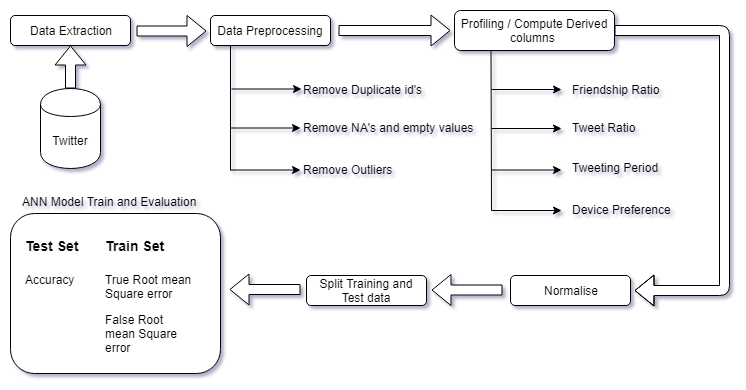
\includegraphics[scale=0.7]{Methodology}
The entire application flow can be summerized using the above flow diagram. First step includes extraction of real world data, we have used python library called 'tweepy' for extracting the data in csv format.\\

The quality of the machine learning algorithm depends directly on the quality of input data, real world data tends to be messy with many missing values, redundant and noisy data etc, hence in the second step we carry out exploratory data analysis where we clean the data looking for missing, NA's or empty values, look for duplicate id's and identify any outliers and remove them since they can make the ANN model unstable for prediction.\\

In the third step we derive the columns like Friendship Ratio, Tweet Ratio, Tweeting Period, Device Preference using the algorithm discussed in section \ref{featureDescription}. The derived values are then normalized to scale within 0 to 1. \\

Once the data is preprocessed and all the derived columns are available, we split the data into train and test data, we use the train data to prepare the ANN model and once the model is trained we use the remaining test data to evaluate the accuracy of the model to test how well the model has learnt from it's test data.


\end{document}